% lecture05.tex — Transversality, Homotopy, and Stability

\section{Transversality}

\begin{definition}{Transversality of Submanifolds}{transversal-submanifolds}
    We say two smooth submanifolds $M, M' \subset N$ are \emph{transversal} at $p \in M \cap M'$ if $T_p M + T_p M' = T_p N$. If they are transversal at every point $p \in M \cap M'$, we simply say they are \emph{transversal}, and write $M \pitchfork M'$.
\end{definition}

\begin{definition}{Transversality of a Map}{transversal-map}
    More generally, we say a smooth map $f \colon M \to N$ is \emph{transversal} to a submanifold $M' \subset N$ (abbreviated $f \pitchfork M'$) if
    \[
        \im(df_p) + T_q M' = T_q N \quad \text{for every } p \in f^{-1}(M'),
    \]
    where $q = f(p)$.
\end{definition}

\begin{center}
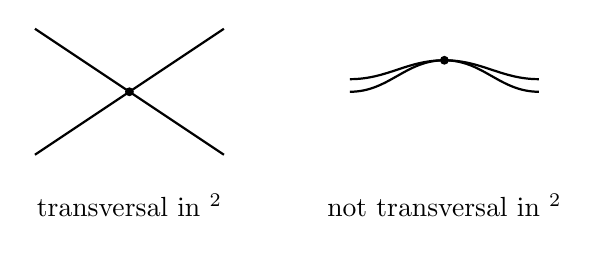
\begin{tikzpicture}[scale=0.8]
    % Transversal
    \draw[thick] (-1.5,-1) -- (1.5,1);
    \draw[thick] (-1.5,1) -- (1.5,-1);
    \fill (0,0) circle (2pt);
    \node at (0,-1.8) {transversal in $\R^2$};
    % Not transversal
    \begin{scope}[xshift=5cm]
        \draw[thick] (-1.5,0) to[out=0,in=180] (0,0.5) to[out=0,in=180] (1.5,0);
        \draw[thick] (-1.5,0.2) to[out=0,in=180] (0,0.5) to[out=0,in=180] (1.5,0.2);
        \fill (0,0.5) circle (2pt);
        \node at (0,-1.8) {not transversal in $\R^2$};
    \end{scope}
\end{tikzpicture}
\end{center}

The following theorem generalizes the preimage theorem for regular values:

\begin{theorem}{Transversal Preimage Theorem}{transversal-preimage}
    If $f \colon M \to N$ is a smooth map transversal to a submanifold $P \subset N$, then the preimage $f^{-1}(P) \subset M$ is a submanifold of $M$, whose codimension (i.e.\ $\dim M - \dim f^{-1}(P)$) equals that of $P \subset N$ (i.e.\ $\dim N - \dim P$).
\end{theorem}

\begin{proof}
    We need to show that every point $p \in f^{-1}(P)$ has a neighborhood $U$ in $M$ such that $f^{-1}(P) \cap U$ is a manifold.

    Let $q = f(p)$. In a neighborhood of $q$, we may write $P$ as the zero set of a collection of independent functions $g_1, \ldots, g_\ell$, where $\ell = \codim P = \dim N - \dim P$.

    \begin{center}
    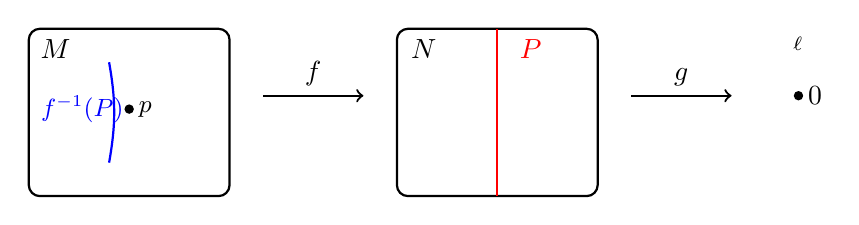
\begin{tikzpicture}[scale=0.85]
        % M with f^{-1}(P)
        \draw[thick,rounded corners] (-1.5,-1) rectangle (1.5,1.5);
        \node at (-1.1,1.2) {$M$};
        \draw[thick,blue] (-0.3,-0.5) to[out=80,in=280] (-0.3,1);
        \node[blue] at (-0.7,0.3) {\small $f^{-1}(P)$};
        \fill (0,0.3) circle (2pt) node[right] {\small $p$};
        % Arrow f
        \draw[->,thick] (2,0.5) -- (3.5,0.5) node[midway,above] {$f$};
        % N with P
        \draw[thick,rounded corners] (4,-1) rectangle (7,1.5);
        \node at (4.4,1.2) {$N$};
        \draw[thick,red] (5.5,-1) -- (5.5,1.5);
        \node[red] at (6,1.2) {$P$};
        % Arrow g
        \draw[->,thick] (7.5,0.5) -- (9,0.5) node[midway,above] {$g$};
        % R^l
        \fill (10,0.5) circle (2pt) node[right] {$0$};
        \node at (10,1.2) {$\R^\ell$};
    \end{tikzpicture}
    \end{center}

    Then, near $p$, $f^{-1}(P)$ is the zero set of $(g_1 \circ f, \ldots, g_\ell \circ f) = g \circ f$, so it's enough to show that $0$ is a regular value of $g \circ f$.

    Since $d(g \circ f)_p = dg_q \circ df_p$ and $dg_q \colon T_q N \to \R^\ell$ is surjective with $\ker dg_q = T_q P \subset T_q N$, $0$ is a regular value of $g \circ f$ if and only if $\im(df_p) + T_q P = T_q N$, which is exactly our transversality assumption.
\end{proof}

\begin{corollary}{Intersection of Transversal Submanifolds}{transversal-intersection}
    If $M, M' \subset N$ are two transversal submanifolds, then $M \cap M'$ is also a submanifold, with
    \[
        \codim(M \cap M') = \codim M + \codim M'.
    \]
\end{corollary}

\begin{remark}{Additivity of Codimension}{codim-additivity}
    Additivity of codimension is very natural. Think: cutting out a submanifold locally using $k = \codim M$ and $\ell = \codim M'$ independent functions.
\end{remark}

\section{Homotopy and Stability}

\begin{definition}{Homotopy}{homotopy}
    We say two smooth maps $f_0, f_1 \colon M \to N$ are \emph{homotopic}, abbreviated $f_0 \sim f_1$, if there exists a smooth map $F \colon M \times I \to N$ such that $F(x,0) = f_0(x)$ and $F(x,1) = f_1(x)$. We call such $F$ a \emph{homotopy} between $f_0$ and $f_1$.

    (Here $f_t(x) = F(x,t)$ is a smoothly evolving family of maps.)
\end{definition}

Homotopy is an equivalence relation on smooth maps from $M$ to $N$, and the equivalence class to which a map belongs is called its \emph{homotopy class}.

\begin{definition}{Stability}{stability}
    A property of smooth maps is called \emph{stable} if whenever $f_0 \colon M \to N$ possesses the property and $f_t \colon M \to N$ is a homotopy of $f_0$, then, for some $\varepsilon > 0$, each $f_t$ with $t < \varepsilon$ also possesses the property.
\end{definition}

\begin{theorem}{Stability Theorem}{stability-thm}
    The following classes of smooth maps of a \emph{compact} manifold $M$ into a manifold $N$ are stable classes:
    \begin{itemize}
        \item local diffeomorphisms,
        \item immersions,
        \item submersions,
        \item maps transversal to a given closed submanifold $P \subset N$,
        \item embeddings,
        \item diffeomorphisms.
    \end{itemize}
    (See Guillemin--Pollack pp.~36--37 for the proofs.)
\end{theorem}
